\documentclass[12pt]{article}
\usepackage[margin=1in]{geometry}
\usepackage{amsmath,amsthm,amssymb,amsfonts}
\usepackage{graphicx}

\newcommand{\N}{\mathbb{N}}
\newcommand{\Z}{\mathbb{Z}}

\newenvironment{problem}[2][Problem]{\begin{trivlist}
\item[\hskip \labelsep {\bfseries #1}\hskip \labelsep {\bfseries #2.}]}{\end{trivlist}}
%If you want to title your bold things something different just make another thing exactly like this but replace "problem" with the name of the thing you want, like theorem or lemma or whatever

\newenvironment{answer}[2][Answer]{\begin{trivlist}
\item[\hskip \labelsep {\bfseries #1}\hskip \labelsep {\bfseries #2.}]}{\end{trivlist}}

\begin{document}

%\renewcommand{\qedsymbol}{\filledbox}
%Good resources for looking up how to do stuff:
%Binary operators: http://www.access2science.com/latex/Binary.html
%General help: http://en.wikibooks.org/wiki/LaTeX/Mathematics
%Or just google stuff

\title{AST 231: Problem Set 6}
\author{Jonas Powell}
\maketitle

\begin{problem}{1}
Pre-main sequence stars in their T Tauri phase are believed to be fully convective and, therefore, they satisfy the equation of state
appropriate to an adiabatic zone through their entire volume. Also, their central densities are not high enough to make degeneracy effects important, so we can assume that the ideal gas law applies. Finally, they are still chemically homogeneous, so we can assume that they have a Population I chemical composition (say, X = 0.73, Y = 0.25 and Z = 0.02) throughout.


\bigskip
\bigskip

With these assumptions, create a stellar model for a pre-main sequence star with characteristics similar to a typical T Tauri star, namely mass = 0.5 solar masses, effective temperature = 4000 K and luminosity = 1 solar luminosity. Plot the density, pressure and temperature of this star as a function of distance from the center.

\bigskip
\bigskip

[Note: While it is true that pressure depends on density to the 5/3 power in this star, just like in the low mass white dwarf, the equation of state is not identical to that case. This star is NOT supported by electron degeneracy and you cannot use the value of K given in Problem Set 6. This question is different, and we have not specified K. Instead we have specified the mass, luminosity and effective temperature that your model must match. It will be acceptable to have a model that comes close to the specified values of mass, temperature and luminosity even if it does not match them precisely.]
\end{problem}






\begin{answer}{1}


\end{answer}

For this problem, we would like to make stellar models that explore $K/\rho_{\text{center}}$ parameter space and find the best values for those variables to return a model star most like the one described in the problem. Since we are given the star's mass, luminosity, and temperature, we are then able to extract its radius and thus do some nice fitting.

\bigskip
\bigskip

To do so, we might use code from the last problem set, but unfortunately for me, since I did end up with a functioning stellar-modeling code, I had to write this one more or less from scratch, in the process transitioning from a homemade integrator to using Scipy's ODE integrator to integrate the equations of hydrostatic equilibrium, mass conservation, and the polytropic equation of state. Testing showed that this integrator worked well, and so I continued on to setting up code to search parameter space.

\bigskip
\bigskip

Finding the most effective path through a wide parameter space to the correct solution is a well-explored area of fitting. One has several options, two of the more famous being a simple grid search and Markov-Chain Monte Carlo (generally implemented using the emcee package). Although I wanted to try implementing an MCMC routine for this problem, I ended up taking a third, simpler route, that of Scipy's optimize.minimize function, which is a wonderful, one-line solver. For my code, I used the Nelder-Mead descent algorithm, since it seemed like the most robust option for my problem.

\bigskip
\bigskip

Using this optimizer, we can loop through test values for $K$ and $\rho_{center}$. In each iteration, I calculate the $\chi^2$ value of the difference between the model and given values of the star's mass and radius, both normalized by their solar values to make them unitless and thus comparable. This $\chi^2$ value is then fed back into the optimizer as it makes its way to the minimum on the $K/\rho_{center} \chi^2$ surface.

To begin the process, we find the star's radius by recalling:

\begin{align}
  L &= 4 \pi r^2 \sigma T_{eff}^4 \\
  r &= \sqrt{\frac{L}{4 \pi \sigma T_{eff}^4}}
\end{align}

From this, we have a "true" value to compare our model radii to of about 20 solar radii.

After running the code for some time, we find that the optimizer settles on $K$ and $\rho_{center}$ values (both reported in MKS units) of:

\begin{align}
  K &= 5.33 \cross 10^{9} \\
  \rho_{center} &= 0.484
\end{align}

which results in stellar mass and radius of

\begin{align}
  M &= 0.499 M_{\odot} \\
  R &= 14.37 R_{\odot}
\end{align}


\bigskip
\bigskip


While the radius is about $25\%$ off of what it should be, we do find that it is in the ballpark of accuracy, and that the reported mass is only thousandths of a solar mass off the correct value. Thus, we trust that while the $K$ and $\rho_{center}$ values that led to those values are slightly off, they are pretty darn close to the correct values.

\bigskip
\bigskip

As a check, we would like to see what the functional forms of the star's pressure, density, and temperature are. Luckily, we have $P(r)$ readily available since it is what we integrated over, and $\rho(r)$ can easily be found by rearranging the polytropic equation of state. However, we must find $T(r)$. We can do this by rearranging the Ideal Gas Law to find:

\begin{align}
  T(r) &= \frac{\rho * \text{mean molecular weight}}{\text{P(r) } K}
\end{align}

From HW4, we know that the mean molecular weight of a star of this composition is 0.6. With this information, we can now plot the desired parameters.

\bigskip
\bigskip

\bigskip
\bigskip


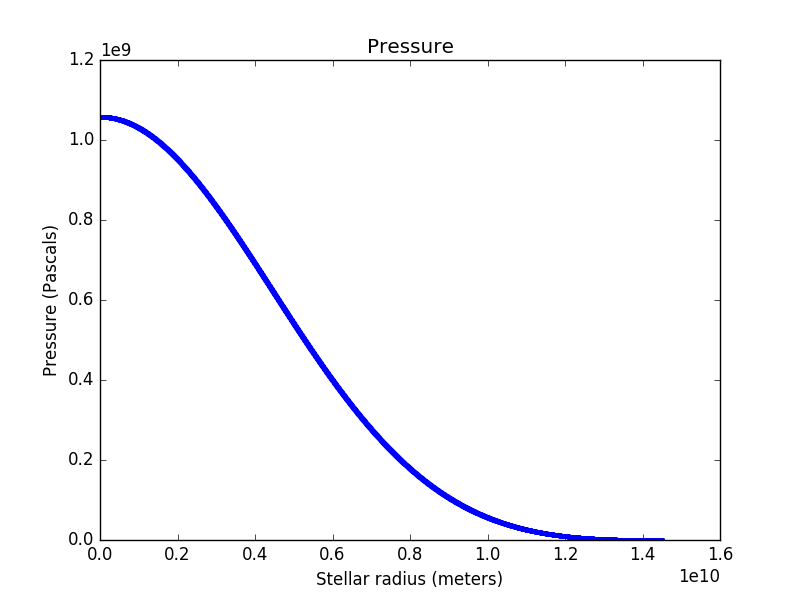
\includegraphics[scale=0.25]{pressure_r.png}
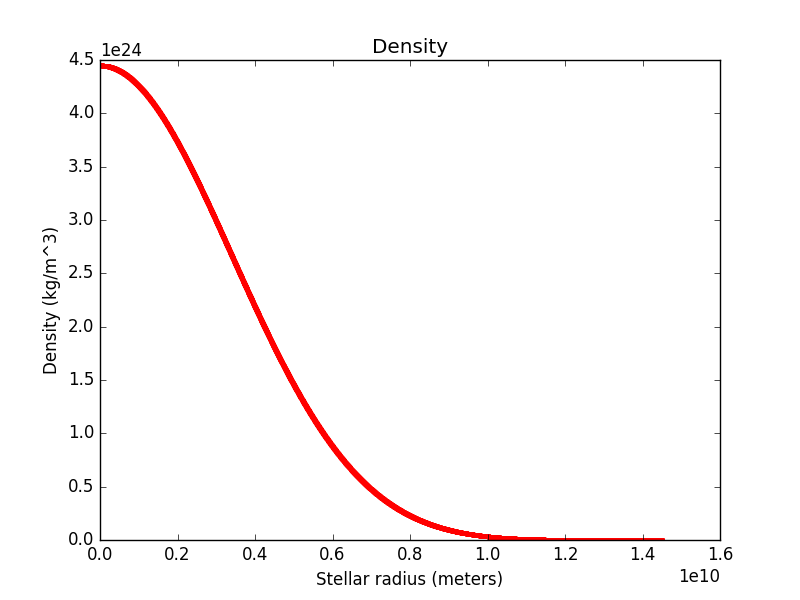
\includegraphics[scale=0.25]{rho_r.png}
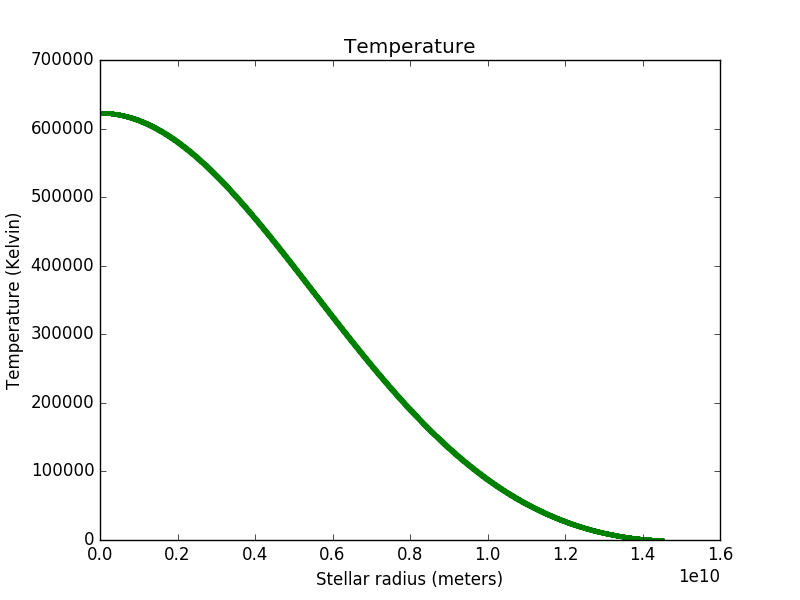
\includegraphics[scale=0.25]{Temperature_r.png} \\


As seen in the figures above, the functional forms of the pressure, temperature, and density structures look reasonable as well.


\end{document}
